%-------------------------------------------------------------------------------
%	SECTION TITLE
%-------------------------------------------------------------------------------
\cvsection{Project Experience}


%-------------------------------------------------------------------------------
%	CONTENT
%-------------------------------------------------------------------------------

%\cvsubsection{Innovative business practices \& Competition}

\begin{cventries}


%---------------------------------------------------------
	\cventry
	{Host} % Job title
	{Smart Image: Medical Image Recognition System based on Federated Learning} % Organization
	{Hainan, China} % Location
	{2020.03 - PRESENT} % Date(s)
	{
		\begin{minipage}[b]{0.25\linewidth}
			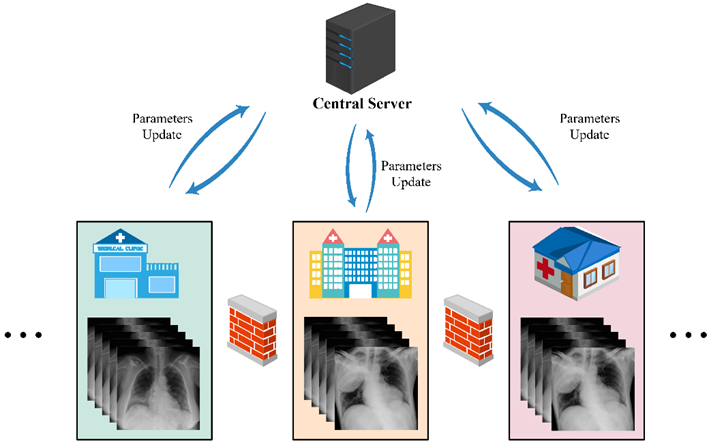
\includegraphics[height=8\baselineskip]{figure/fedcov.png}
		\end{minipage}
		\hfill
		\begin{minipage}[b]{0.7\linewidth}
			% 我们设计了一款基于联邦学习的医疗影像识别软件,可以在保护患者数据隐私的前提下进行多方联合。在数据方面,我们汇总了网上的多个公开数据集,并用Pydicom将dicom文件转换成图片形式用于模型识别。在模型方面,我们将包括ResNet、COVID-Net在内的4个模型进行模型融合,增强系统稳定性和泛化能力。同时,我们用GradCAM++对卷积层进行可视化,用于标记病灶位点,最后能够自动化生成医学报告。另外,在多方贡献衡量方面我们提出了FedCM贡献评估算法。
			We designed a medical image recognition software based on federated learning that allows for multi-party federation while protecting the privacy of patient data. In the aspect of data, we aggregate several published datasets on the Internet. In terms of models, we fused four models including ResNet and COVID-Net for model fusion to enhance system stability and generalization capability. We use GradCAM++ to visualize the convolutional layers for annotating lesion sites, and finally the software can generate medical reports automatically. In addition, we propose the FedCM contribution evaluation algorithm in the multiparty contribution measurement. \textcolor{awesome-red}{\href{https://github.com/beiyuouo/paddle-fl-gui}{[Code]}}
		\end{minipage}
	}

%---------------------------------------------------------
	\cventry
	{Participate} % Job title
	{5G Road Patrol Car} % Organization
	{Hainan, China} % Location
	{2020.05 - PRESENT} % Date(s)
	{
		\begin{minipage}[b]{0.25\linewidth}
			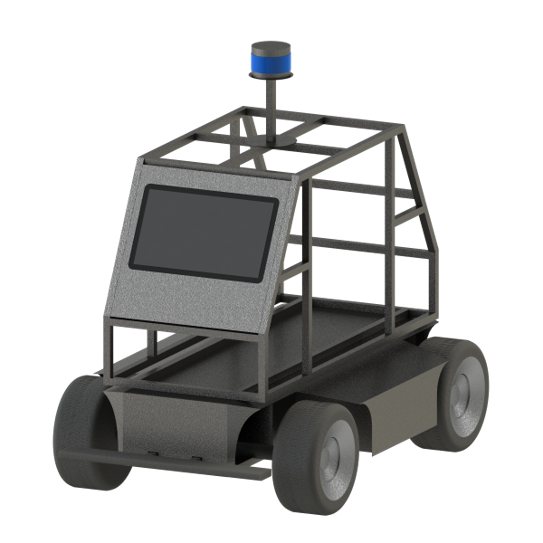
\includegraphics[height=8\baselineskip]{figure/car.png}
		\end{minipage}
		\hfill
		\begin{minipage}[b]{0.7\linewidth}
			% 我们设计了一款基于5G和多传感器融合用于城市巡逻的无人路检机器人,主要功能有基于多传感器融合的道路裂缝、坑洼等缺陷检测并进行云端上报,和违停检测。在建图和定位方面,我们基于LeGO-LOAM进行调整和改进。在道路检测方面,我们基于Yolov5训练了自己的模型,F1-score达到了0.68
			We designed an unmanned road inspection robot based on 5G and multi-sensor fusion for city patrol. The main functions are multi-sensor fusion-based detection of road cracks, potholes and other defects and reporting them to the cloud, and parking violation detection. For mapping and localization, we adapt and improve the algorithm based on LeGO-LOAM. For road detection, we have trained our own model based on Yolov5, and the F1-score reached 0.68.
		\end{minipage}
	}

%---------------------------------------------------------
  \cventry
    {Participate} % Job title
    {ROV technology-based underwater sightseeing robot.} % Organization
    {China} % Location
    {2020.05 - PRESENT} % Date(s)
    {
      This is a national student innovation and entrepreneurship project. We use underwater ROV for image collection and transmission. After defogging, we perform stitching of video frame sequences to achieve panoramic landscape viewing.
    }

%---------------------------------------------------------
%\end{cventries}

%\cvsubsection{Open Source Project}

%\begin{cventries}
%---------------------------------------------------------
%	\cventry
%	{Owner} % Job title
%	{FedMedical:PaddleFL-based Federated Learning Medical Image Recognition Software} % Organization
%	{\href{https://github.com/beiyuouo/paddle-fl-gui}{\color{awesome-red}{[GitHub link]}}} % Location
%	{2020.11 - PRESENT} % Date(s)
%	{
%		\begin{cvitems} % Description(s) of tasks/responsibilities
%			\item {Distributed Deployment and Federated Learning Simultaneous Training with PaddleFL Framework.}
%		\end{cvitems}
%	}

%---------------------------------------------------------
	\cventry
	{Owner} % Job title
	{Mid-air Draw: Gesture Recognition and Tracking based on YOLOv5} % Organization
	{Hainan, China} % Location
	{2020.09 - PRESENT} % Date(s)
	{
		We label the data ourselves and use YOLOv5 for gesture recognition and finger key point recognition. It is able to interact with PPT and other software to achieve the function of mid-air drawing. \textcolor{awesome-red}{\href{https://github.com/beiyuouo/mid-air-draw}{[Code]}} \textcolor{awesome-red}{\href{https://www.bilibili.com/video/BV15V411a7WB/}{[Video]}}
	}

	
%---------------------------------------------------------
\end{cventries}

